\newpage
\begin{minipage}[b]{0.40\textwidth}
	\normalsize \textbf{\qquad2.} %жирный текст
	Р е ш е н и е.    Пусть \textit{ОС} -- медиана\\
	треугольника \textit{OAB$_1$}
        (рис 1.).На продолжении\\
	отрезка \textit{OC} за точку \textit{С} возьмем точку \textit{D} так,\\

	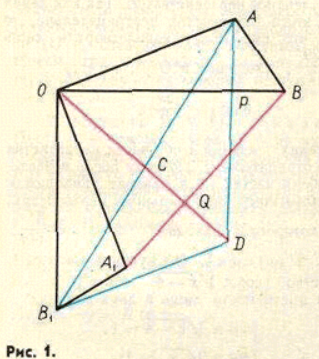
\includegraphics[width=7.5cm]{Lab7_1.png}\\

	\normalsize что \textit{ОС =OD}; тогда \textit{OB$_1$DA} -- параллело-\\
	грамм. Поскольку \textit{ОА = ОА$_1$, AD = OB$_1$} =\\
	= \textit{OB} и  \textit{$\angle$ OAD = $\angle$ A$_1$OB} (как углы в соот-\\
	ветственно перпендикулярными сторонами),\\
	то \textit{$\triangle$AOD = $\triangle$A$_1$OB}. Далее,  \textit{$\triangle$OPA} =\\
	=  \textit{$\triangle$OQA$_1$}, а \textit{$\angle$APO = 90$^\circ$ (ибо AD$\|$OB$_1$,\\
	а OB$_1$ $\bot$OB)}; поэтому \textit{OC$\bot$A$_1$B}. Аналогично\\
	доказывается и второе утверждение задачи \\
	\hphantom \qquad  \textbf{3.} \textit{x$_1$ = 3, y$_1$ = ( 2k + 1 )$\pi$}, где \textit{k} = 0, \\
	\textit{$\pm$1, $\pm$2, . . ., 0 < x$_2$ < 1, y$_2$}  - любое ве -\\
	щественное число. \quad У к а з а н и е.  Пусть\\
	\textbf{z} = \textit{log$_3$x}; тогда предложенное неравенство\\
	записывается в виде

	\begin{equation}
		 z+\frac{1}{z}\ll -2\cos{y} 
	\end{equation}

	Но при любом z> 0 имеем \textit{$ z+\frac{1}{z}\geq 2$}, а\\
	потому неравенство (1)   может  быть спра -\\
	ведливым только для тех y, для которых \textit{2$\ll$ \\
	$\ll$-2\quad$\cos{y}$}, то есть при \textit{$\cos{y}$ = -1}. Да - \\
	лее, из (1) получаем \textit{z} = 1. Если же \textit{z} < 0,\\
	то  \textit{$ z+\frac{1}{z}\quad \ll \quad -2$,\quad а -2 $\ll$ -2 $\cos{y}$} при\\
	любом y, то есть неравенство (1) справед-\\
	ливо при всех \textit{z} < 0\\
	\hphantom \qquad \textbf{4.}Решение существует, если \textit{b} < -1,\\
	а \textit{$\alpha$} -- любое действительное число, или если\\
	\textit{b $\geq$ -1}, а\\

	\textit{$\kappa \pi$ -- $\arcsin{A+\phi}$ $\ll \alpha\ll\kappa \pi+$} 
	\begin{equation}
		+ \arcsin{A + \phi}, \kappa = 0, \pm 1, \pm 2, ...,
	\end{equation}
	\textit{где А и $\phi$ определяются равенствами}
	\begin{equation}
		 \tg{\phi} = \frac{b+1}{2}, A = \frac{|b - 1|}{\sqrt{b^2+2b+5}}.
	\end{equation}
		
\end{minipage}
\begin{minipage}[b]{0.60\textwidth}
	\normalsize \qquad\qquad \quad У к а з а н и е. Так как \textit{x $\neq \frac{\pi}{2}(2\kappa+1)$,\\
	\hphantom\qquad\qquad y $\neq \frac{\pi}{2}(2\kappa+1)$}, то исходная система эквива -\\
	\hphantom\qquad\qquad лентна следующей (проверьте!):\\
	\hphantom\qquad\qquad \[\left\{
	\hphantom\qquad\qquad \begin{aligned}
	x + y =\alpha\\
	2\sin{(x+y)}-(b-1)\cos{(x+y)} =\\
	= (b-1) \cos{(x-y)}
	\hphantom\qquad\qquad  \end{aligned}\right.
	\hphantom\qquad\qquad \]

	\hphantom\qquad\qquad Следовательно, исходная система имеет ре-\\
	\hphantom\qquad\qquad шение тогда и только тогда, когда\\
	\hphantom\qquad\qquad \textit{(b-1)$\cos{(x-y)}$ = 2$\sin{\alpha}$ - (b+1)$\cos{\alpha}$}.(4)\\
	\hphantom\qquad\qquad Если \textit{b$\neq$1}, то из (4) получаем, что параметры\\
	\hphantom\qquad\qquad \textit{a и b} должны удовлетворять условию\\
	\begin{equation*}
		|\frac{2\sin{a}-(b+1)\cos{a}}{b-1}| \ll 1.
	\end{equation*}
	\hphantom\qquad\qquad Вводя \textit{$\phi$ и А} по формулам (3), это условие\\
	\hphantom\qquad\qquad представим в виде \textit{|$\sin{\alpha - \phi}\ll$A}. Та-\\
	\hphantom\qquad\qquad ким образом, либо\textit{ А} > 1 ( то есть \textit{b} < -1)\\
	\hphantom\qquad\qquad и \textit{$\alpha$} -- любое действительное, либо \\
	\hphantom\qquad\qquad \textit{А} $\ll$ 1  (то есть \textit{b $\geq$ -1, b $\neq$ 1)}, а для \textit{$\alpha$} по-\\
	\hphantom\qquad\qquad лучаются неравенства (2). В случае \textit{b =1} \\
	\hphantom\qquad\qquad соотношение (4) исследуется непосредственно.
	
	\begin{center}
		\textbf{Физический факультет}\\
	\end{center}

	\hphantom\qquad\qquad \qquad\quad \textbf{1.}  $\frac{{q^m}^n - 1}{(q^n - 1) {q^(m-1)}^n}$.  У к а з  а н и е. За-\\
	\hphantom\qquad\qquad метьте, что если \textit{$\nu$} -- средняя скорость на\\
	\hphantom\qquad\qquad перегоне \textit{$A_1$$A_2$} после отправления, то на\\
	\hphantom\qquad\qquad перегоне \textit{$A_n$$A_1$}, завершаюшем первый круг,\\
	\hphantom\qquad\qquad средняя скорость равна \textit{$\nu^{(n-1)}$},  а на пере-\\
	\hphantom\qquad\qquad гоне  \textit{$A_1$$A_2$}, открывающем второй круг, она\\
	\hphantom\qquad\qquad равна  \textit{$\nu^n$}.

	\hphantom\qquad\qquad \qquad\quad \textbf{2.} \textit{ $r^2$ cosec $\alpha \sin{\beta} \sin2(\alpha+\beta)\cos(\alpha$+\\
	\hphantom\qquad\qquad +$\beta$)}. У к а  з а н и е. Рассмотреть отдельно \\
	\hphantom\qquad\qquad случаи, когда \textit{$\angle$ODB > $\angle$MDB $\angle$ODB <\\
	\hphantom\qquad\qquad < $\angle$MDB},  где О -- центр круга.

	\hphantom\qquad\qquad \qquad\quad \textbf{3.} x > 2.

	\hphantom\qquad\qquad \qquad \textbf{4.} \textit{$\frac{1}{12}$$\ll$ a $\ll$ $\frac{1}{2}$;\\
	\hphantom\qquad\qquad \quad x =$(-1)^n$ $\arcsin\frac{5\alpha\pm\sqrt{\alpha^2 + 4\alpha}}{2\alpha}$ + $\kappa\pi$,\\
	\hphantom\qquad\qquad \qquad \qquad $\kappa$ = 0, $\pm$ 1, $\pm$ 2}, ...

	\begin{center}
		\textcolor{blue}{ МОСКОВСКИЙ\\
		ИНЖЕНЕРНО-ФИЗИЧЕСКИЙ ИНСТИТУТ}
	\end{center}
	
	\begin{center}
		 \textit{ В а р и а н т 1}
	\end{center}

	\hphantom\qquad\qquad \qquad \textbf{1.} 23. Р е ш е н и е. Искомое число за-\\
	\hphantom\qquad\qquad пишем в виде 1\textit{0х + у}, где \textit{х и у} -- целые\\
	\hphantom\qquad\qquad числа, причем \textit{1$\ll$x$\ll$9, 0$\ll$y$\ll$9}. Так\\
	\hphantom\qquad\qquad как по условию при делении двузначного чис-\\
	\hphantom\qquad\qquad ла на \textit{ху} получили остаток, равный 5, то \textit{ху$\neq$0};\\
	\hphantom\qquad\qquad следовательно, \textit{1$\ll$y$\ll$9}. Из условия за\\
	\hphantom\qquad\qquad дачи получим систему

	 \[\left\{
	 \begin{aligned}
		\frac{10x+y}{x+y}&=4+\frac{3}{x+y},\\
		\frac{10x+y}{xy}&=3+\frac{5}{xy}.
	\end{aligned}\right.
	\]
	\hphantom\quad\\

\end{minipage}

\newpage
\begin{minipage}[b]{0.42\textwidth}
	\normalsize Подставляя t = 37, 38, 39, 40, 41 в формулы\\
	(*) получаем 5 вариантов:\\
 
\begin{tabular}{ | l | l | l | l | l | l | }
\hline
батарей & 34 & 26 & 18 & 10 & 2\\
по 6 в & \hspace{0pt} & \hspace{0pt} & \hspace{0pt} & \hspace{0pt} & \hspace{0pt}  \\ \hline
батарей  & 1 & 4 & 7 & 10 & 13\\
по 16 в & \hspace{0pt} & \hspace{0pt} & \hspace{0pt} & \hspace{0pt} & \hspace{0pt} \\ 
\hline
\end{tabular}
	
	\normalsize \textit \\\\{б) Здесь дело водится к решению урав-\\
	нения 6х + 15у = 220. Однако НОД (6,15) =\\
	= 3, а 220 не делится на 3. Поэтому урав-\\
	нение не имеет решений в целых числах.}
	\hphantom\qquad \textbf{19.} Сумма четного числа нечетных чисел\\
	четна, поэтому 45 рублей нельзя разменять\\
	указанным способом.\\
	\hphantom\qquad \textbf{20.} Поскольку \textit{a = bd} и делится на \textit{с},\\
	а НОД \textit{(b,c)} = 1, то по лемме 3 число \textit{d}\\
	делится на c.\\
	\hphantom\qquad \textbf{21.} a), б) и г) верны; б) неверно.\\
	\hphantom\qquad \textbf{22.} 1971 = $3^3$*43; 1972 = 4 * 17 * 29;\\
	1973 -- простое.\\
	\hphantom\qquad \textbf{23.} а) если \textit{am}  делится на \textit{n} и\\
	НОД (m,n) = 1, то \textit{a = $\kappa$n}, поэтому \textit{b =$\kappa$m}.\\
	\hphantom\qquad б) пусть в разложении х на простые мно-\\
	жители некоторое простое \textit{р} входит в степени\\
	\textit{$\alpha$}, а в разложении \textit{у} -- то же \textit{р} в степени \textit{b}.\\
	Тогда из теоремы о единственности разло-\\
	жения на простые множители  \textit{a = $\kappa$n},  \textit{b =$\kappa$m}.\\
	В разложении \textit{t} на простые множители вклю-\\
	чим \textit{p} с показателем \textit{k}, и так  -- для всех про-
	стых множителей чисел \textit{x} и \textit{y}.\\
		
\end{minipage}
\begin{minipage}[b]{0.62\textwidth}
	\normalsize \hphantom\qquad\qquad непосредственным вычислением показать, что\\
	\hphantom\qquad\qquad \textit{AQ = $\alpha$}\\
	\hphantom\qquad\qquad \hphantom\qquad \textbf{5.} \textit{d$\sqrt{\kappa}$}. У к а з а н и е. Убедиться, что\\
	\hphantom\qquad\qquad $\triangle$ \textit{MQE} $\sim$ $\triangle$ \textit{PNE}, причем \textit{EM и EP} -- сход-\\
	\hphantom\qquad\qquad ственные стороны.

	\begin{center}
		\textbf{Факультет психологии}\\
	\end{center}

	\hphantom\qquad\qquad \hphantom\qquad \textbf{1.} 3.\\
	\hphantom\qquad\qquad \hphantom\qquad \textbf{2.} Точка \textit{P} должна совпадать либо с\\
	\hphantom\qquad\qquad \hphantom\qquad вершиной \textit{C}, либо с вершиной \textit{$C_1$}.\\
	\hphantom\qquad\qquad \hphantom\qquad \textbf{3.} $-\frac{1}{\sqrt{2}}<x<0$.\\
	\hphantom\qquad\qquad \hphantom\qquad \textbf{4.} 11 деьалей вида \textit{A}, 9 деталей вида \textit{B}.\\
	\hphantom\qquad\qquad \hphantom\qquad \textbf{5.} \textit{a} = 1.

	\begin{center}
		\textbf{МОСКОВСКИЙ ИНСТИТУТ\\
		ИНЖЕНЕРОВ ЖЕЛЕЗНОДОРОЖНОГО\\
		ТРАНСПОРТА}\\
	\end{center}

	\hphantom\qquad\qquad \hphantom\qquad \textbf{1.} За 30 дней.\\
	\hphantom\qquad\qquad \hphantom\qquad \textbf{2.} $x_1$ = 0, $x_2$ = -2, \qquad ${x_3}_4$ = -1 $\pm$\\
	\hphantom\qquad\qquad $\pm\sqrt{\frac{33}{2}}$.\\
	\hphantom\qquad\qquad \hphantom\qquad \textbf{3.} \textit{r} = $\frac{25}{4}$\textit{см.}\\
	\\
	\\
	\\
	\\
	\\
	\\
	\\	
	\\
\end{minipage}
